\documentclass[12pt]{article}%

\usepackage{fancyhdr}
\pagestyle{fancy}
\fancyhf{}
\fancyhead[R]{\thepage}

\usepackage{cmap}				
\usepackage{mathtext} 
\usepackage{listings}

\usepackage{biblatex}
\addbibresource{lib.bib}

\usepackage{euscript}
\usepackage{mathrsfs}

\usepackage[T2A]{fontenc}
\usepackage[utf8]{inputenc}
\usepackage[english,russian]{babel}
\usepackage{amsmath,amsfonts,amssymb,amsthm,mathtools}

\setlength\fboxsep{3pt}
\setlength\fboxrule{1pt}

\usepackage{graphicx}
\usepackage{hyperref}
\usepackage[usenames,dvipsnames,svgnames,table,rgb]{xcolor}
\usepackage{wrapfig}
\hypersetup{				
    unicode=true,           
    pdftitle={Заголовок},   
    pdfsubject={Тема},      
    pdfkeywords={keyword1} {key2} {key3},
    colorlinks=true,
    linkcolor=black,
    citecolor=black,
    filecolor=magenta,
    urlcolor=cyan
}

% Работа с Python
\usepackage{minted}
\definecolor{LightGray}{gray}{0.98}

% Работа с enumerate
\usepackage{enumitem}

\newcommand*{\Title}{\begingroup
\centering 

\large {Федеральное автономное образовательное учреждение высшего образования}
\vspace*{\baselineskip}

\large {«Национальный исследовательский университет «Высшая школа экономики»»}
\vspace*{\baselineskip}

\vspace*{\baselineskip}
\large{\textbf{Отчет по лабораторной работе 3}}

\vspace{0.1cm}
\large{Решение систем алгебраических уравнений итерационными методами}

\vspace{0.2cm}
\large{Вариант 10: задачи 4.1.10, 4.5.3, 5.1.10, 5.4.4}

\vspace{1.5cm} 

\begin{flushright}
  \textbf{\normalsize Выполнил:}
  
  \vspace{0.3cm} 
  {\normalsize Студент группы БПМ-211}
  
  {\normalsize Ляхов Артём Андреевич}

\end{flushright}


\vspace{0.2cm}  
\begin{flushright}
  \textbf{\normalsize Преподаватель:} 

  \vspace{0.2cm}

 {\normalsize Брандышев Петр Евгеньевич}
 
\end{flushright}

\vfill
\date{}{Март 2024 г.}


\endgroup\clearpage}

\begin{document}
\Title
\tableofcontents

\newpage

\section{Задача 4.1.10 Решение системы нелинейных уравнений методом Ньютона}
\subsection{Формулировка задачи}
Требуется, используя метод Ньютона, найти с точностью $\varepsilon = 10^{-6}$ все корни системы нелинейных алгебраических уравнений:
\begin{equation}\label{task1:cond}
    \begin{cases}
        f_1(x_1, x_2) = 0 \\
        f_2(x_1, x_2) = 0
    \end{cases}
    \begin{cases}
        \sin(x_1 + x_2) - x_2 - 1.5 = 0 \\
        x_1 + \cos(x_2 - 0.5) - 0.5 = 0
    \end{cases}
\end{equation}

\subsection{Теоретический материал}
Пусть дана система из $n$ нелинейных уравнений с $n$ неизвестными:
\begin{equation}\label{task1:eq1}
    \begin{cases}
        f_1(x_1, \dots, x_n) = 0  \\
        f_2(x_1, \dots, x_n) = 0  \\
        \dots \\
        f_n(x_1, \dots, x_n) = 0
    \end{cases}
\end{equation}
где $f_i(x_1, x_2, \dots x_n)$, $i = 1,\dots, n$ - непрерывно дифференцируемые в некоторой области $G \subset \mathbb{R}^n$ функции.

Обозначим за $F(x) = (f_1(x)\ \dots\ f_n(x))^T$, $x \in \mathbb{R}^n$. Пусть $x^{(k)}$ - $k$-ое приближение решения системы \ref{task1:eq1}. Построим линейную аппроксимацию $F(x)$ в окрестности точки $x^k$:
\begin{equation}\label{task1:eq2}
    F(x^{(k+1)}) \approx F(x^{(k)})\ +\ W(x^{(k)})(x^{(k+1)} - x^{(k)}) = 0
\end{equation}
где $W$ - матрица Якоби:
\begin{equation*}
W = 
\begin{pmatrix}
    \frac{\partial f_1}{\partial x_1} & \dots & 
    \frac{\partial f1}{\partial x_n} \\
    \dots & \dots & \dots \\
    \frac{\partial f_n}{\partial x_1} & \dots &
    \frac{\partial f_n}{\partial x_n}
\end{pmatrix}
\end{equation*}

Решим систему \ref{task1:eq2} относительно $x^{k+1}$, в результате чего получим итеративный метод, называемый \textit{методом Ньютона}:
\begin{equation}
    x^{(k+1)} = x^{(k)} - W^{-1}(x^{(k)}) F(x^{(k)})
\end{equation}

Вычисление обратной матрицы - сложная вычислительная задача. Для того, чтобы избежать этого введём обозначение $y^{(k)} = W^{-1}(x^{(k)})F(x^{(k)})$, тогда $y^{(k)}$ в виде решения системы линейных уравнений:
\begin{equation*}
    W(x^{(k)}) \cdot y^{(k)} = F(x^{(k)}) 
\end{equation*}

Тогда шаг метода Ньютона можно переписать в следующем виде:
\begin{equation}
    \begin{cases}
        W(x^{(k)}) \cdot y^{(k)} = F(x^{(k)}) \\
        x^{(k+1)} = x^{(k)} - y^{(k)}
    \end{cases}
\end{equation}

\subsection{Порядок решения задачи}
\begin{enumerate}
    \item Используя встроенные функции, локализуем корни системы уравнений графически.
    \item Напишем функцию, вычисляющую корень системы двух нелинейных уравнений по методу Ньютона с точностью $\varepsilon$.
    \item Используя вышеуказанную функцию, вычислим все корни заданной системы с точностью $\varepsilon$. 
    \item Найдём корни системы, используя встроенную функцию, и сравним с результатом полученным в третем пункте.
\end{enumerate}

В качестве критерия окончания итеративного процесса чаще всего использую условие $||x^{(k+1)} - x^{(k)}|| < \varepsilon$.

При этом если $F(x) \in C^2(G)$, то имеет место \textit{квадратичная сходимость} метода Ньютона.

\subsection{Результаты}
\subsubsection{Графическая локализация корней}
\begin{figure}[h]
    \centering
    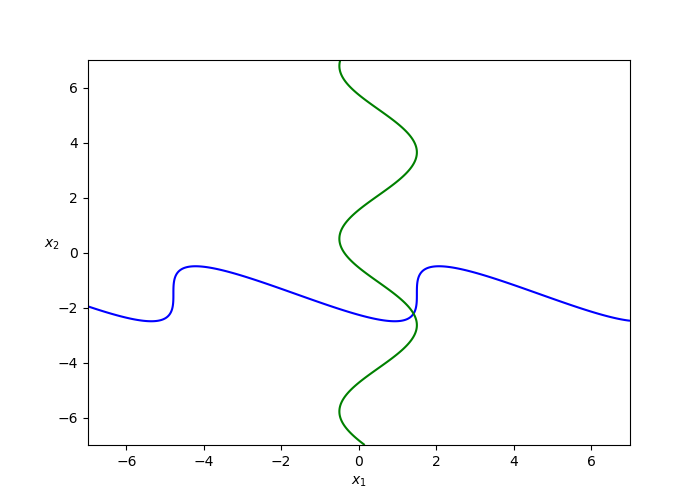
\includegraphics[width=0.8\linewidth]{roots_loc.png}
    \caption{Графическая локализация корня системы уравнений \ref{task1:cond}. Синим изображена линия уровня $f_1(x) = 0$, зелёным - линия уровня $f_2(x) = 0$.}
\end{figure}
\newpage

\subsubsection{Вычисление корней}
\begin{table}[!h]
    \centering
    \begin{tabular}{|c|c|c|}
    \hline
    Начальная точка & Решение методом Ньютона & Решение SciPy \\
    \hline
    (-2.0, 0.0) & (1.41423304, -2.22440735) & (1.41423304, -2.22440735) \\
    \hline
    (1.0, -1.5) & (1.41423304, -2.22440735) & (1.41423304, -2.22440735) \\
    \hline
    \end{tabular}
    \caption{Результаты вычисления корней с помощью реализованного метода и встроенной функции для двух начальных точек. Для первой точки метод Ньютона сошёлся за \textit{7 итераций}, для второй - за \textit{5 итераций}. Для обеих начальных точек абсолютная погрешность решений составила порядка $1.49 \cdot 10^{-9}$.}
    \label{tab:my_label}
\end{table}

\textbf{Вывод:} как мы видим, реализованная нами программа находит решение с погрешностью, не превосходящей $10^{-8}$.

\newpage
\section{Задача 4.5.3 Нахождение ближайшей точки к поверхности}
\subsection{Формулировка задачи}
Даны координаты точек $P_1, P_2, P_3$:
\begin{equation*}
    \begin{cases}
        P_1 = (15.5,\ 6.4,\ 12.162) \\
        P_2 = (8.22,\ 5.879,\ 9.122) \\
        P_3 = (14.531,\ 3.464,\ 5.375) 
    \end{cases}
\end{equation*}
и уравнение поверхности $S$:
\begin{equation*}
    \frac{(x_1)^2}{a_1} + \frac{(x_2)^2}{a_2} = 2x_3
\end{equation*}
где $a_1 = 8.5 - 3\times0.25 = 7.75$, $a_2 = 2.3 + 3\times0.3 = 3.2$.

Необходимо определить ближайшую к поверхности точку и наиболее удалённую от поверхности точку. После этого построить на одном чертеже точечный график поверхности $S$ и точки $P_1, P_2, P_3$.

\subsection{Теоретическая часть}
\subsubsection{Метод Ньютона для задачи оптимизации}
Рассмотрим задачу безусловной оптимизации:
\begin{equation*}
    \min\limits_{x \in \mathbb{R}^n}f(x)
\end{equation*}
где $f(x)$ - дважды непрерывно-дифференцируемая функция.

Пусть $x^k$ - $k$-ое приближение точки минимума. Воспользуемся разложением функции $f(x)$ в окрестности точки $x^k$:
\begin{equation}\label{task2:eq1}
    f(x^k + h) \approx f(x^k) + f'(x^k)h + \frac{1}{2}h^T \cdot f''(x^k) h
\end{equation}
где $f'(x^k)$ - градиент, $f''(x^k)$ - гессиан функции $f(x)$ в точке $x^k$.

Поскольку мы хотим найти $h$ такое, что \ref{task2:eq1} достигает минимума, то мы можем найти градиент функции $f(x^k + h)$ по $h$ и прировнять его к нулю. Положив, вместе с тем $x^{k+1} = x^k + h$ мы приходим к соотношению:
\begin{equation}
    x^{k+1} = x^k - \left[f''(x^k) \right]^{-1} f'(x^k)
\end{equation}

Как и в предыдущем случае, мы не будем вычислять явно обратную матрицу, вместо этого к итерации метода добавим решение системы уравнений:
\begin{equation}
    \begin{cases}
        f''(x^k) \cdot y^k = f'(x^k) \\
        x^{k+1} = x^{k} - y^k
    \end{cases}
\end{equation}

Вместе с этим сделаем замечание, что если $f(x)$ не выпукла, то метод Ньютона может сходиться к локальному минимуму, поэтому в дальнейшем при решении мы будем использовать несколько начальных точек $x^0$.

\subsubsection{Расстояние от точки до поверхности}
Пусть $p = (p_1, p_2, p_3)$, $q = (q_1, q_2, q_3)$, $p, q \in \mathbb{R}^3$, введём функцию $H$ как:
\begin{equation*}
H(p, q) = \sum_{i=1}^3\left(p_i - q_i\right)^2 = 
\rho^2(p, q) = ||p - q||^2_2
\end{equation*}

Задачу нахождения расстояния от фиксированной точки до поверхности можно сформулировать в виде задачи условной оптимизации:
\begin{equation*}
    \rho(P_i, S) = \min_{x \in S}\rho(P_i, x)
\end{equation*}
Вместе с тем, минимум функции $\rho$ достигается тогда и только тогда, когда достигается минимум функции $H$, то нам необходимо решить задачу оптимизации для функции $H$:
\begin{equation*}
    \min_{x \in S}H(P_i, x)
\end{equation*}

Однако в нашем случае эта задача очень просто сводится к задаче \textit{безусловной} оптимизации. Для этого достаточно параметризовать поверхность $S$:
\begin{equation*}
    x = x(u, \theta) = 
    \begin{cases}
        x_1 = \sqrt{a_1} \cdot u \cdot \cos(\theta) \\
        x_2 = \sqrt{a_2} \cdot u \cdot \sin(\theta) \\
        x_3 = 0.5 \cdot u^2
    \end{cases}
\end{equation*}

В этом случае параметры $u$ и $\theta$ могут принимать любые значения. Следовательно, мы можем переформулировать задачу нахождения расстояния от фиксированной точки $P_i$ до поверхности $S$ в виде задачи безусловной оптимизации:
\begin{equation*}
    \rho(P_i, S) = \min_{u, \theta}\rho(P_i, x(u, \theta))
\end{equation*}

А как мы поняли до этого, такая задача эквивалентна решению оптимизационной задачи для функции $H$:
\begin{equation*}
    \min_{u, \theta}H(P_i, x(u, \theta))
\end{equation*}

\subsection{Порядок решения задачи}
\begin{enumerate}
    \item Напишем функцию, которая будет с помощью метода Ньютона минимизировать целевую функцию.
    \item С помощью функции из предыдущего пункта и найдём расстояния от точек $P_i$ до поверхности $S$. Чтобы исключить попадание в локальный минимум, будем производить перебор по сетке множества начальных точек.
    \item Графически изобразим поверхность $P$ и точки $P_1, P_2, P_3$ на одном графике.
\end{enumerate}

\subsection{Результаты}
\subsubsection{Результаты вычислений}
\begin{table}[!h]
    \centering
    \begin{tabular}{|c|c|}
    \hline Точка & Расстояние до $S$ \\
    \hline $P_1 = (15.5, 6.4, 12.162)  $  & 3.6474 \\
    \hline $P_2 = (8.22, 5.879, 9.122) $  & 0.2754 \\
    \hline $P_3 = (14.531, 3.464, 5.375)$ & 4.8716 \\
    \hline
    \end{tabular}
    \caption{Результаты вычислений расстояний между поверхностью $S$ и точками $P_1, P_2, P_3$ с использованием метода Ньютона.}
    \label{tab:my_label}
\end{table}

\textbf{Вывод:} таким образом, наименее удалённой от $S$ точкой оказалась $P_2$, а наиболее удалённой - $P_3$.

\subsubsection{Изображение поверхности и точек}
\newpage
\begin{figure}[h]
    \centering
    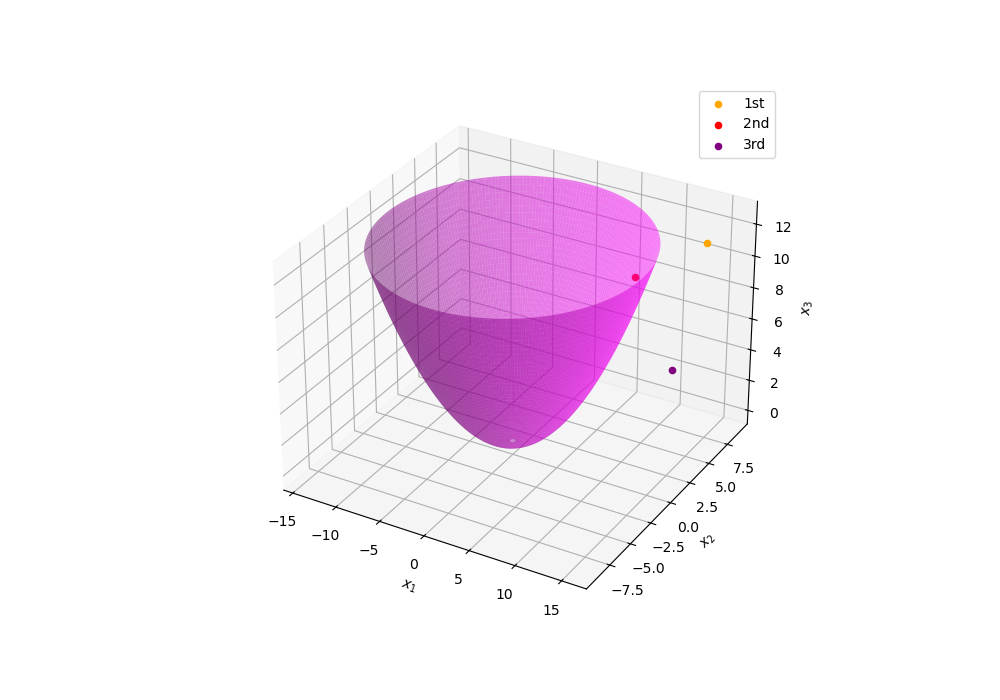
\includegraphics[width=0.95\linewidth]{surface_distance.png}
    \caption{Графическое изображение точек $P_i,\ i \in \{1, 2, 3\}$ и поверхности $S$.}
    \label{fig:enter-label}
\end{figure}


\newpage
\section{Задача 5.1.10 Нахождение решения СЛАУ методом Зейделя}
\subsection{Формулировка задачи}

Дана системы $Ax=b$. Требуется найте решение данной системы с помощью метода Гаусса. Выполнить 10 итераций по методу Зейделя. После этого, принимая решение с помощью метода Гаусса за точное, найти абсолютную погрешность итерационного решения.

\begin{equation*}
A = \begin{pmatrix}
    49.5 & 12.52 & 16.12 & 19.80 \\
    0 & 27.1 & 1.64 & 23.76 \\
    12.87 & 11.52 & 40 & -14.85 \\
    0 & 4.32 & 0.12 & 6.27
\end{pmatrix}
\ \ \ \ \
b = \begin{pmatrix}
-92.98 \\ 25.46 \\ -26.76 \\ -1.15
\end{pmatrix}
\end{equation*}

\subsection{Теоретический материал}
Систему уравнений вида $Ax=b$ можно преобразовать к виду $x = Bx + c$, который являтеся очень удобным для применения итерационных методов с помощью следующих соотношений:
\begin{equation}
    \begin{cases}
        b_{ij} = -\frac{a_{ij}}{a_{ii}},\ \ \ i \ne j \\
        b_{ij} = 0,\ \ \ i = j \\
        c_{i} = \frac{b_i}{a_{ii}}
    \end{cases}
\end{equation}

В дальнейшем метод Зейделя сводится к итеративному приближению решения $Ax=b$ посредством соотношения
\begin{equation}
    x^{k+1} = Bx^k + c,
\end{equation}
где $x^k$ - $k$-ое приближение решения.

Отметим при этом, что далеко не всегда данный итеративный метод сходится. Достаточным условием сходимости итерационных методов, которым мы будем пользоваться при решении, является условие $||B||_{\infty} < 1$.

\subsection{Порядок решения задачи}
\begin{enumerate}
    \item Задать матрицу системы $A$ и вектор правой части $b$. Найти решение системы $Ax=b$ с помощью метода Гаусса.
    \item Преобразовать систему $Ax=b$ к виду $x = Bx+c$, удобному для итераций. Проверить выполнение достаточного условия сходимости итерационных методов $||B||_{\infty} < 1$.
    \item Написать функцию, которая решает систему по методу Зейделя. Взять любое начальное приближение и сделать 10 итераций по этому методу. Найти абсолютную погрешность, принимая решения, полученное в пункте 1 за точное.
    \item Взять другое начальное приближение и проделать ещё раз все вышеуказанные операции. 
\end{enumerate}

\subsection{Результаты вычислений}
\begin{table}[h]
    \centering
    \begin{tabular}{|c|c|c|c|}
         \hline $x_1$ & $x_2$ & $x_3$ & $x_4$   \\
         \hline -1.101 & 3 & -2 & -2.2121 \\
         \hline
    \end{tabular}
    \caption{Решение системы $Ax=b$ с помощью метода Гаусса. Это решение принимается за точное.}
\end{table}

\begin{table}[h]
\centering
\begin{tabular}{|c|c|c|c|c|c|}
\hline $x^0$ & $x_1$ & $x_2$ & $x_3$ & $x_4$ & $\varepsilon$ \\
\hline $(0, 0, 0, 0)$ & -1.2549 & 2.7015 & -1.7338 & -1.9861 & 0.2985 \\
\hline $(1, 1, 1, 1)$ & -1.1651 & 2.7979 & -1.6921 & -1.8861 & 0.3260 \\
\hline
\end{tabular}
\caption{Приближённые решения системы уравнений после 10 итераций по методу Зейделя. $x^0$ - вектор начального приближения, $\varepsilon$ - абсолютная погрешность.}
\end{table}

\textbf{Вывод:} Мы видим, что вне зависимости от начального приближения метод Зейделя сходится к точному решению, однако при этом скорость сходимости за 10 итераций для разных начальных приближений может отличаться.  



\newpage
\section{Задача 5.4.4 Исследование зависимости решения СЛАУ итерационным методом от параметра}
\subsection{Формулировка задачи}
Дана система уравнений $x = Bx + c$, где $B = B(t)$, 
$t = -1, -0.8, \dots, 0.8, 1$ - параметр. 

Необходимо:
\begin{enumerate}
    \item Построить график (или гистрограмму) зависимости нормы $||B||_{\infty}$ от параметра $t$. По этому графику определить, при каких $t$ выполнено достаточное условие сходимости итерационных методов.
    \item Для наибольшего из значений $t$, при которых выполнено условие сходимости, решить с точностью $\varepsilon = 10^{-5}$ систему $x = Bx + c$.
\end{enumerate}

Матрица $B$ и вектор $c$ задаются в виде:
\begin{equation*}
B = \begin{pmatrix}
    -0.2 & \cos(3t) & 0.1 & 0.3 \\
    0.1 & 0.11 & 0.4 & -0.05 \\
    0.3 & 0.1 & \sin(3t) + \cos(2t) & 0.1 \\
    0.2 & -0.12 & 0.1 & 0.09
\end{pmatrix}
\ \ \ \ \
b = \begin{pmatrix}
0 \\ 1 \\ 2 \\ 3
\end{pmatrix}
\end{equation*}

\subsection{Результаты}
\subsubsection{График зависимости нормы матрицы $B$}
\begin{figure}[h]
    \centering
    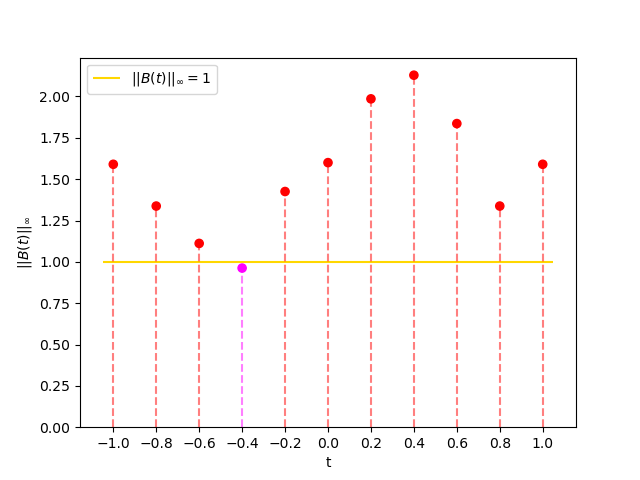
\includegraphics[width=0.9\linewidth]{matrix_norm.png}
    \caption{График зависимости $\infty$-нормы матрицы $B$ от параметра $t$.}
\end{figure}

\newpage
\textbf{Вывод:} только для значения $t = -0.4$ выполнено достаточное условие сходимости итерационных методов. Таким образом, в дальнейшем мы будем искать решение системы для $t = -0.4$. 

\subsubsection{Решение системы}
\begin{table}[h]
    \centering
    \begin{tabular}{|c|c|c|c|}
    \hline $x_1$ & $x_2$ & $x_3$ & $x_4$ \\
    \hline 1.81394 & 2.26257 & 2.54025 & 3.67616 \\
    \hline
    \end{tabular}
    \caption{Решение системы $x = B(t) x + c$ для $t=-0.4$. Для нахождения решения использовался метод Зейделя. В качестве критерия остановки использовалось условие $||x^{k+1} - x^{k}||_{\infty} < \frac{\varepsilon}{2}$, где $\varepsilon = 10^{-5}$ - точность.}
\end{table}

\section{Приложение}
Все вычисления в рамках решения задач лабораторной работы проводились на языке Python (версия 3.11) с помощью пакета NumPy и пакета Autograd, который предоставляет набор инструментов для автоматического дифференцирования.

Код для проведения вычислений можно найти в прикреплённом вместе с отчётом ноутбуке lab3.ipynb.

\end{document}